%% example for producing articles in MVA format using LaTeX.
%% written by Takeshi MASUDA, Electrotechnical Laboratory, Japan in May 1996.
%% modified by KAGESAWA Masataka, OKAZAKI Shin'ichro, YASUMOTO Mamoru.
%% last modified by Masaki Onishi, AIST, in Nov 2012.
%% use at your own risk.

\documentclass{mva_style}
\usepackage{graphicx}
\usepackage{amsmath,amssymb, yhmath,bm} % for expectation sign
\DeclareMathOperator*{\argmax}{arg\,max} \DeclareMathOperator*{\argmin}{arg\,min}
\usepackage{microtype}

\finalcopy %Uncomment this line for the Camera-Ready Manuscript

\begin{document}
\title{Optimization-based Brush Style Transfer with Feedforward Neural Networks}

\author{
  Saki Kohata\\
  Waseda University\\
  Tokyo\\
  {\tt cat-73@akane.waseda.jp}\\
  \and
  Edgar Simo-Serra\\
  Waseda University\\
  Tokyo\\
  {\tt ess@waseda.jp}\\
}

\maketitle

\section*{\centering Abstract}
\textit{
Style transfer has emerged as a powerful way to perform advanced edits to
images to match the style of a source image and has become a staple tool in
artistic creation. However, such style transfer is usually treated as an
image-to-image translation problem, where a myriad of losses and
hyper-parameters are used for the user to attempt to modify a desired content
image into the style of another style image.
Instead of basing our approach on an image-to-image translation model, we
leverage stroke based optimization approaches to learn an accurate stroke
representation of the style image, and then repaint the content image using the
learned stroke representation to reproduce it in the different style.
Our approach is more flexible and interpretable than existing image-to-image
based approaches, potentially opening up many different interactive usage
scenarios.
  %The emergence of machine learning has revolutionized the world of digital 
  %art, providing people with the ability to create highly polished images 
  %without advanced drawing skills. 
  %However, most approaches focus o
  %However, most of the studies that have been conducted to generate pictures 
  %using machine learning are not tools that can be used by people who are 
  %already working as creators, such as changing images to artistic styles or 
  %generating images based on text. In this study, we propose a model that 
  %learns brush styles of human paintings and generates new input images that 
  %are redrawn using the learned brush styles. 
  % ess: don't write limitations in the abstract
  %The generated images by the proposed model are not perfect imitations of 
  %the brush style of the reference image. This is thought to be caused by 
  %the limitation of the model to generate flexible strokes due to minimal 
  %stroke parameters.
  % Our model has the potential to significantly streamline the process of picture creation for creators, offering a powerful new tool for artists and designers alike.
}


\section{Introduction}
It is said that in order for people to paint a good picture, they need 
to master many techniques, which takes a long time. However, with the 
advancements in machine learning, it is now possible for people without 
painting skills to generate high-quality paintings. 
For example, Midjourney\cite{Midjourney} is a software application that 
allows users to create wonderful paintings by simply entering words, 
sentences, or keywords that describe the image they wish to have painted. 
However, it is difficult to say that such a tool is useful for creators who 
have already established their own style. For creators, it is important to 
create works by their own hands, whether digital or analog, and a tool like 
Midjourney, which relies on machine learning for the entire picture creation 
process, is likely to leave creators dissatisfied with the shape and color 
of the drawn objects. Therefore, we aim to conduct research that can support 
creators during their work. Our goal is to develop a model that learns the 
brush style of a picture drawn by a creator and adapts the brush style to a 
new image. In this study, we propose a model that takes two input images, 
a content reference image and a style reference image, and generates an image 
in which what was drawn in the content reference image is redrawn with the 
brush style of the style reference image. 
Figure {fig:haru} shows examples of two input images and an output image.
The picture shown in the content reference image was created with a solid 
coloring brush, so the boundary between colors is always clear. The picture 
shown in the style reference image was created using a brush with a texture 
similar to that of an analog picture, so it is possible to make a gradation 
between colors. The generated image is a 
representation of the one drawn in the content reference image with the 
brush style of the style reference image.
It is expected that creators can greatly streamline the process of creating 
pictures by manually creating images like the content reference image shown 
in Figure\ref{fig:haru} using a simple brush, and then inputting it into the 
model to have it redrawn with the creator's brush style. Since the content 
reference image is created by the creator, the shape and color of the object 
can be controlled by the creator, and any dissatisfaction with the generated 
image can be resolved with some modifications.

\begin{figure}[ht!]
  \centering
  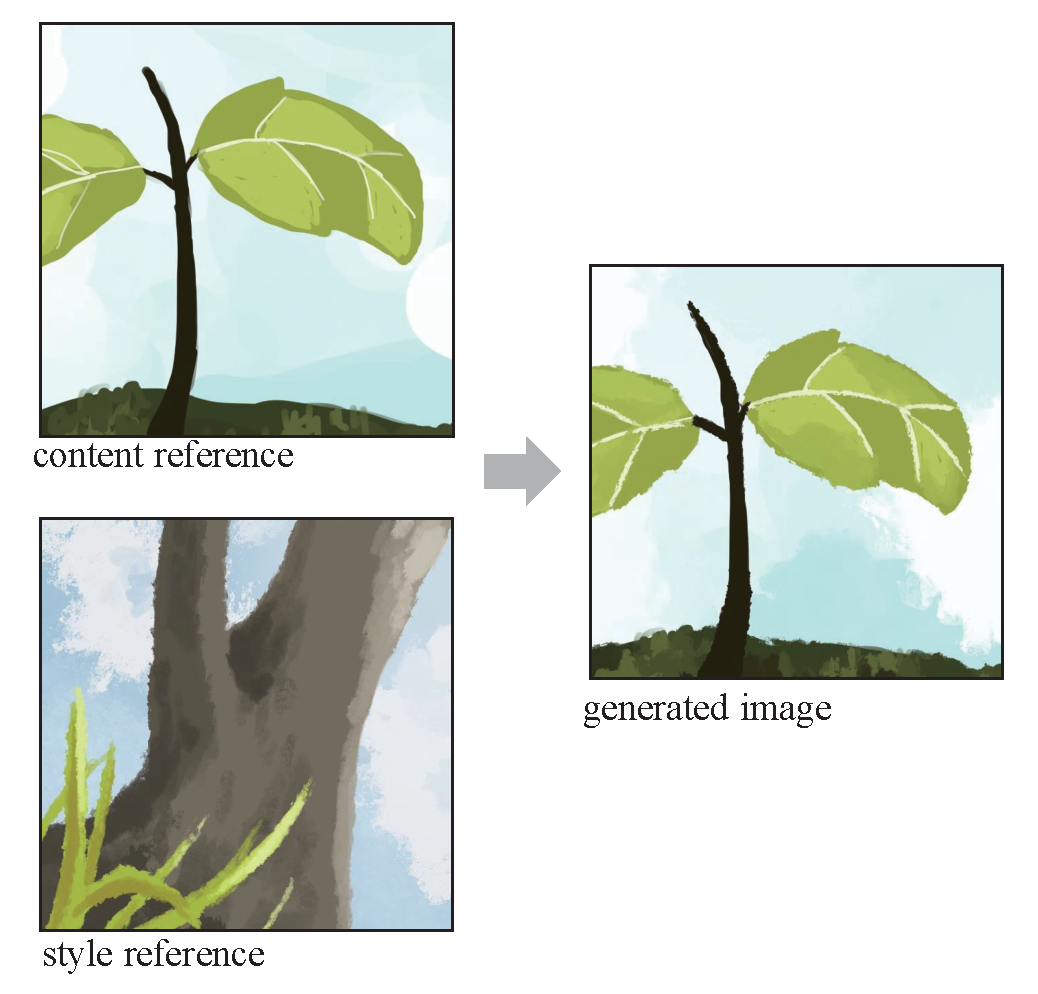
\includegraphics[width=83mm]{resource/haru.eps}
  \caption{Example of the goal of our research, where we wish to create a new image using the style and content of separate reference images.}
  \label{fig:haru}
\end{figure}

\begin{figure*}[t]
  \centering
  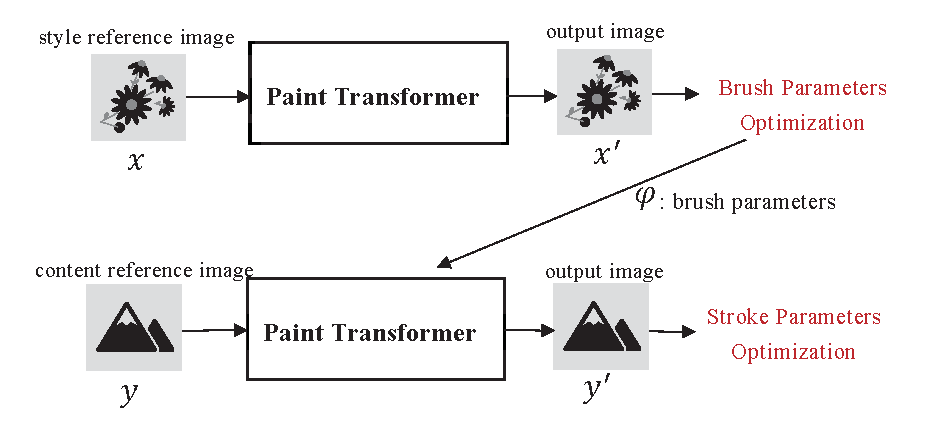
\includegraphics[width=166mm]{resource/target_model.eps}
  \caption{Overview of our proposed model architecture. We first learn a stroke representation $s^g$ from the style image via optimization, and then apply the learnt representation to modify the content image.}
  \label{fig:final_model}
\end{figure*}


\section{Related Work}
The use of machine learning to generate paintings has been heavily researched 
and has made significant progress. The method using neural networks as a 
generative tool is typically formulated as a pixel-wise mapping \cite{PerceptualLosses} 
or a continuous optimization process in pixel space \cite{ImageStyleTransfer}.
However, it is difficult for a neural network to imitate the process that a 
human draws. Humans typically start 
by applying rough colors and then gradually adding details, while neural 
networks generate images pixel by pixel. To imitate the human drawing 
process, the machine would have the ability to decompose a given image into 
an ordered sequence of strokes. While neural networks can create sketches 
\cite{DBLP:journals/corr/HaE17}, \cite{DBLP:journals/corr/abs-1805-00247} 
and doodles \cite{DBLP:journals/corr/abs-1810-05977} with a small number of 
strokes, creating a texture-rich painting requires many more strokes.
This makes it difficult to set loss functions for each stroke and prepare 
ground-truth strokes. As a result, Reinforcement Learning (RL) is often used 
to decompose strokes in texture-rich images. \cite{DBLP:journals/corr/abs-1804-01118, DBLP:journals/corr/abs-1206-4634, Huang_2019_ICCV}
Because the computational cost is high in the learning process of an RL agent, 
there are also studies that have formulated this process as a stroke 
parameter search. \cite{PaintTransformer}
The brush style transfers addressed in this paper are similar to those 
addressed in Neural Style Transfer \cite{ImageStyleTransfer}, in which the 
overall mood of an input style image (such as a painting) is transferred to 
another image, using CNNs. The model proposed in that study can transform a 
landscape photograph into an artistic style, but the atmosphere and colors of 
the style reference image as a whole are transferred to the content reference 
image. Therefore, characteristic objects depicted in the style reference 
image, which are not present in the content reference image, appear in the 
output image from the model. 
In this study, we aim to only transfer the style of the brush without changing 
the contents and colors drawn in the content reference image. We addressed 
this issue by adopting the Transformer-based stroke generation pipeline 
proposed by Liu \textit{et al.}~\cite{PaintTransformer} as a stroke prediction 
model for our proposed model.

\section{Proposed Approach}

Our approach consists of first finding a set of strokes $S_l$ and stroke style
$\hat{s}_g$ that can represent a style image $I_{style}$. Afterwards, we then fix the
stroke style $\hat{s}_g$ and find another set of strokes $S_l'$ to represent the
content image with the style of the reference style image.
An overview of our approach is shown in Figure \ref{fig:final_model}.

\subsection{Framework}

Our approach is built around a stroke prediction model $M$ that is able to
recreate an image from a set of strokes $S_l$ and stroke style $s_g$.
We first find a stroke style $\hat{s}_g$ by minimizing a loss function $L$ that
measures the error between the stroke prediction model $M$ and target style
image $I_{style}$:
\begin{equation}
  \hat{s}_g = \argmin_{s_g} \;
      \min_{S_l} \;
         L\left( M\left(S_l, s_g\right), I_{style}\right)
  \label{eq_first}
\end{equation}
Afterwards, we fix the stroke style $\hat{s}_g$ and again minimize the stroke
prediction error, but this time measured with the target content image
$I_{comment}$:
\begin{equation}
  \hat{S}_l = \argmin_{S_l} (L(M(S_l, \hat{s}_g), I_{content}))
  \label{eq_second}
\end{equation}
This resulting output image then simply computed by using the stroke prediction
model with the optimal strokes $\hat{S}_l$ and stroke style $\hat{s}_g$:
\begin{equation}
   I_{output} = M( \hat{S}_l, \hat{s}_g )
\end{equation}

\subsection{Stroke Prediction Model}

We utilize the Transformer-based framework called Paint Transformer proposed by
Liu \textit{et al.}~\cite{PaintTransformer} as our stroke prediction model $M$.
Paint Transformer is a Transformed-based framework that generates a sequence of
strokes using a forward propagating transformer.  Paint Transformer consists of
two modules: a stroke predictor and a stroke renderer. 
A stroke consists of eight parameters: center coordinates $x$, $y$, height $h$,
width $w$, rotation angle $\theta$, and $r$, $g$, $b$ corresponding to RGB values 
representing colors, respectively. Each stroke $s$ can be expressed as $s = \{ x,
y, h, w, \theta, r, g, b \}$. The strokes rendered by Paint
Transformer are based on monochromatic strokes that are scaled and rotated from the base
brush image and given colour. Paint Transformer generates multiple strokes based on eight
randomly generated parameters and uses them as a training dataset to train a
stroke predictor. Since the training dataset is generated randomly and
automatically, there is no need to prepare a dataset. 

\subsection{Stroke Styles}

\begin{figure}
  \centering
  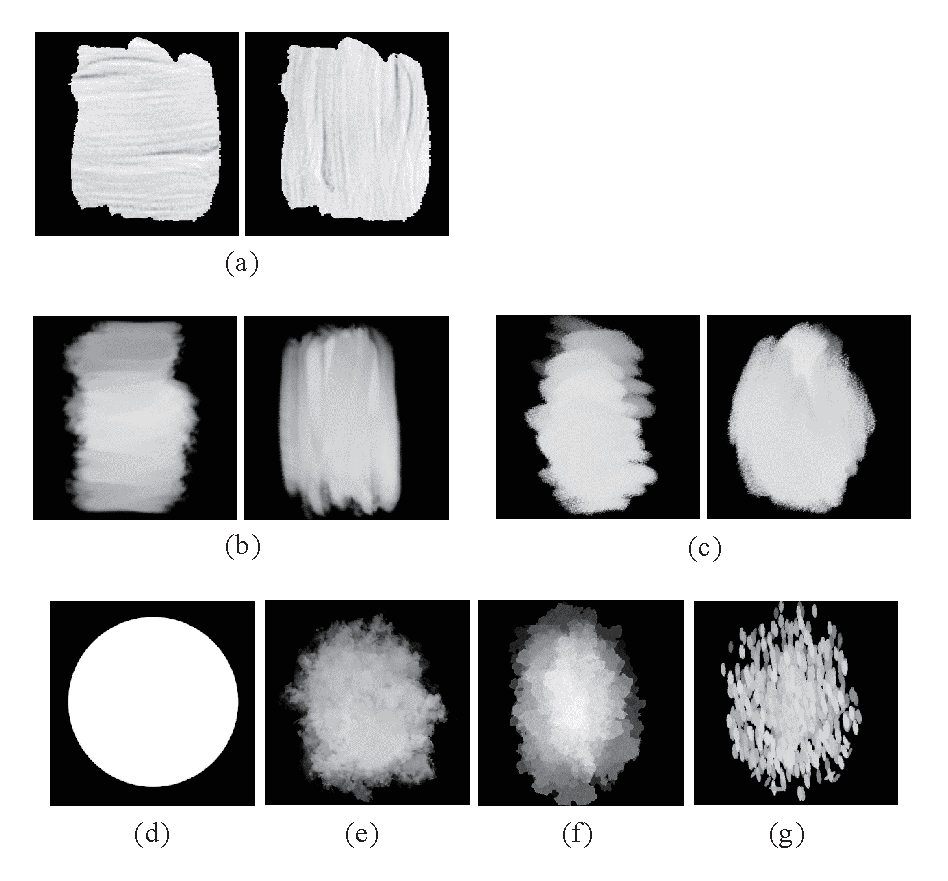
\includegraphics[width=80mm]{resource/brushes.eps}
  \caption{Diversity of brushes used in this work for more accurate representation of painting styles.}
  \label{fig:brushes}
\end{figure}

Paint Transformer used a single brush image to generate strokes. 
We newly created six types of brush images. Figure \ref{fig:brushes} shows 
the seven brush images. (a) is the brush image used by Liu \textit{et al.} and (b)-(g) 
are the newly created ones. In (a)-(c), brush images are provided separately for
horizontal and vertical strokes.
% \begin{equation}
%   \phi = \mathop{\rm argmin}\limits_{\phi}(\mathop{\rm argmin}\limits_{e}(L(x^{\prime}, x)) + R(e))
% \end{equation}

% Here, $L$ is the content loss and $R$ is the stroke regularization term. By 
% inputting a style reference image $x$ as a content reference image into the 
% Paint Transformer and obtaining the result $x^{\prime}$, we can determine the 
% optimal stroke parameters $e$ and then use them, along with the regularization term, 
% to determine the optimal brush parameters $\phi$.
% Next, the content reference image is input to Paint Transformer. At this time, 
% the brush parameters optimized earlier are used. The output is used to optimize 
% the stroke parameters. The optimization of the stroke parameters is performed 
% using the following equation.

% \begin{equation}
%   e = \mathop{\rm argmin}\limits_{e}(L(y^{\prime}, y) + \psi(x, y^{\prime}))
% \end{equation}

% Here, $L$ is the content loss and $\psi$ is the style loss. These are used to 
% find the optimal stroke parameters $e$.
% The above two optimizations are repeated alternately to bring the brush and 
% stroke parameters closer to the optimum.


% \subsection{Structure of the proposed model}
% As mentioned earlier, double optimization has not been implemented at this 
% stage. In the proposed model, multiple base brush images are prepared, and 
% the final output image is the one with the highest similarity of brush style 
% with the style reference image among the results of multiple runs of Paint 
% Transformer using those images. 
% Paint Transformer is used for the stroke prediction model, and a function to 
% evaluate the similarity of the style with the style reference image is added 
% to the part after stroke prediction by Paint Transformer using the seven 
% types of brush images described below.

\begin{figure}[t]
  \centering
  \includegraphics[width=80mm]{resource/dataset.eps}
  \caption{Content reference image and style reference image used in the experiment.}
  \label{fig:inputs}
\end{figure}

% \subsection{Loss Function}
% The $L1$ loss of the Gram matrix is employed as a loss function to evaluate 
% the brush style of the output image generated by the Paint Transformer and 
% the style reference image. We judged that the Gram matrix is suitable for 
% the evaluation of brush styles because it allows us to consider a wide range 
% of image correlations.

\begin{figure}[t]
  \centering
  \includegraphics[width=80mm]{resource/results.eps}
  \caption{(a) Style reference image input to the model and a partially enlarged image of the output from the model.
           (b) Output image from Neural Style Transfer~\cite{ImageStyleTransfer}.
           The content and style reference images are (a) and (c) in Figure \ref{fig:inputs}, respectively.
         }
  \label{fig:result}
\end{figure}

\begin{figure}[t]
  \centering
  
\includegraphics[width=80mm]{resource/brush_discussion.eps}
  \caption{Images of the brushes used in the proposed model (left), 
  strokes drawn using Clip Studio Paint (upper right), 
  and a brush image stretched to match the strokes drawn in Clip Studio Paint (lower right).}
  \label{fig:discussion}
\end{figure}

\section{Experiments and Results}

\subsection{Experiments}
The proposed model takes a content reference image and a style reference image, 
and outputs a result image. For the content images, we used one cat image from 
The Oxford-IIIT Pet Dataset \cite{oxford-dataset}.
The content reference image and style reference image used are shown in Figure \ref{fig:inputs}.
Image (b) is \textit{Composition with Red,
Blue, and Yellow} by Piet Mondrian, 1930. Image (c) is \textit{The Starry Night} 
by Vincent van Gogh, 1889.

\subsection{Results}
When the seven brush images shown in Figure \ref{fig:brushes} were used to 
generate strokes that represent the content reference image shown in Figure 
\ref{fig:inputs}, the image with the highest similarity to the style reference 
image is shown in (a) of Figure \ref{fig:result}. 
These brush styles are not very similar, which can be attributed to the fact 
that there were only seven base brush images and the parameters used to represent 
the strokes were minimal. It can be confirmed that the content of the output 
image has not changed significantly from that of the content reference image.
Image \ref{fig:result}, (b) is the output image obtained when the content 
reference image is inputted to Neural Style Transfer \cite{ImageStyleTransfer}.
The brush style is imitated 
with high accuracy, but the color has changed from the original content 
reference image and the stars drawn in the style reference image have appeared.

\section{Discussion and Limitations}
In this study, we proposed a novel approach to transform the content of a 
content reference image into a style that imitates the brush style of a style 
reference image using a forward propagating neural network. 
We used a Transformer-based framework called Paint Transformer to redraw the 
content drawn in the content reference image using the brush style of the 
style reference image. In the proposed model, since the stroke 
prediction model was trained using Paint Transformer as it is, the stroke 
parameters are the same as those of Paint Transformer, \textit{i.e.}, five shape 
parameters and three color parameters, for a total of eight. In future studies, 
we believe that adding more parameters will enable more flexible brush stroke 
representation. The strokes generated by the proposed model are created by 
scaling and rotating the brush images shown in Figure\ref{fig:brushes}, but 
strokes can also be generated by connecting multiple brush images in 
succession. For example, CLIP STUDIO PAINT \cite{ClipStudio}, a paint software, 
can draw strokes as shown in the upper right of Figure\ref{fig:discussion}, but simply 
adjusting the size of the brush image cannot generate similar strokes, 
resulting in strokes like the one shown in the lower right of Figure\ref{fig:discussion}.
It is expected that by increasing the number of stroke parameters, we can 
increase the expressiveness of the brush and generate strokes like the one 
in the upper right of Figure\ref{fig:discussion}, which imitate the brush style of the 
style reference image. 


\begin{thebibliography}{99}
\bibitem{Midjourney}
“Midjourney,” Accessed: 2023-01-09. [Online]. Available: https://midjourney.com/.

\bibitem{PerceptualLosses}\sloppy
J. Johnson, A. Alahi, and L. Fei-Fei, “Perceptual losses for real-time
style transfer and super-resolution,” \textit{CoRR}, vol. abs/1603.08155, 2016.
arXiv: 1603 . 08155. [Online]. Available: http://arxiv.org/abs/1603.08155.

\bibitem{ImageStyleTransfer}
L. A. Gatys, A. S. Ecker, and M. Bethge, “Image style transfer using
convolutional neural networks,” in \textit{Proceedings of the IEEE Conference
on Computer Vision and Pattern Recognition (CVPR)}, Jun. 2016.

\bibitem{DBLP:journals/corr/HaE17}\sloppy
D. Ha and D. Eck, “A neural representation of sketch drawings,” \textit{CoRR},
vol. abs/1704.03477, 2017. arXiv: 1704 . 03477. [Online]. Available:
http://arxiv.org/abs/1704.03477.

\bibitem{DBLP:journals/corr/abs-1805-00247}
J. Song, K. Pang, Y. Song, T. Xiang, and T. M. Hospedales, “Learning
to sketch with shortcut cycle consistency,” \textit{CoRR}, vol. abs/1805.00247,
2018. arXiv: 1805.00247. [Online]. Available: http://arxiv.org/abs/
1805.00247.

\bibitem{DBLP:journals/corr/abs-1810-05977}
T. Zhou, C. Fang, Z. Wang, J. Yang, B. Kim, Z. Chen, J. Brandt,
and D. Terzopoulos, “Learning to sketch with deep q networks and
demonstrated strokes,” \textit{CoRR}, vol. abs/1810.05977, 2018. arXiv: 1810.
05977. [Online]. Available: http://arxiv.org/abs/1810.05977.

\bibitem{DBLP:journals/corr/abs-1804-01118}
Y. Ganin, T. Kulkarni, I. Babuschkin, S. M. A. Eslami, and O. Vinyals,
“Synthesizing programs for images using reinforced adversarial learn
ing,” \textit{CoRR}, vol. abs/1804.01118, 2018. arXiv: 1804.01118. [Online].
Available: http://arxiv.org/abs/1804.01118.

\bibitem{DBLP:journals/corr/abs-1206-4634}
N. Xie, H. Hachiya, and M. Sugiyama, “Artist agent: A reinforcement
learning approach to automatic stroke generation in oriental ink paint
ing,” \textit{CoRR}, vol. abs/1206.4634, 2012. arXiv: 1206 . 4634. [Online].
Available: http://arxiv.org/abs/1206.4634.

\bibitem{Huang_2019_ICCV}
Z. Huang, W. Heng, and S. Zhou, “Learning to paint with model-based
deep reinforcement learning,” in \textit{Proceedings of the IEEE/CVF Inter
national Conference on Computer Vision (ICCV)}, Oct. 2019.

\bibitem{PaintTransformer}
S. Liu, T. Lin, D. He, F. Li, R. Deng, X. Li, E. Ding, and H. Wang,
“Paint transformer: Feed forward neural painting with stroke predic
tion,” in \textit{Proceedings of the IEEE International Conference on Com
puter Vision}, 2021.


\bibitem{ClipStudio}
“CLIP STUDIO PAINT,” Accessed: 2023-01-09. [Online]. Available: https://www.clipstudio.net/.

\bibitem{oxford-dataset}
O. M. Parkhi, A. Vedaldi, A. Zisserman, and C. V. Jawahar, “The
oxford-iiit pet dataset,” [Online]. Available: https://www.robots.ox.ac.uk/~vgg/data/pets/.

\end{thebibliography}



\end{document}
